\chapter{SYSTEM STUDY AND DESIGN}

\section{Core Design Principles}
The design of the \textbf{CNN - FitnessTracker} is guided by the following principles to ensure automated analysis remains stable, portable, and trustable:
\begin{table}[h]
\centering
\begin{tabular}{|p{3.5cm}|p{12.3cm}|}
\hline
\textbf{Principle} & \textbf{Description} \\ \hline
Single Source of Truth & Local coordinate calculations and state variables are managed by the active Flask server thread; the React frontend reflects this data dynamically without running separate calculations. \\ \hline
Coordinate Separation & The display-space (pixels), the normalized 2D screen coordinate space ($0.0$ to $1.0$), and the 3D world coordinate space are kept strictly separate to prevent scaling issues across devices. \\ \hline
Confirmed Irreversibility & Sessions that write or clear logs, reset workout history, or modify rep counts require user confirmations to prevent accidental loss of data. \\ \hline
Fast Visual Feedback & Every movement phase (UP/DOWN/HOLD) triggers instant feedback on the screen via colored overlays and sound effects. \\ \hline
Robust Error Recovery & If the camera feed fails, or the flask connection drops, the system displays user-friendly messages and resumes connection attempts automatically. \\ \hline
\end{tabular}
\caption{System Core Design Principles.}
\label{tab:core_design_principles}
\end{table}

\section{System Architecture}
The system is structured in four cooperating layers: a Presentation layer (React components), a Control/State management layer (React state hooks), a Service layer (Flask computer vision server + MediaPipe), and a Data layer (1D-CNN + LSTM weights, logs, and video storage). 

\begin{figure}[h]
\centering
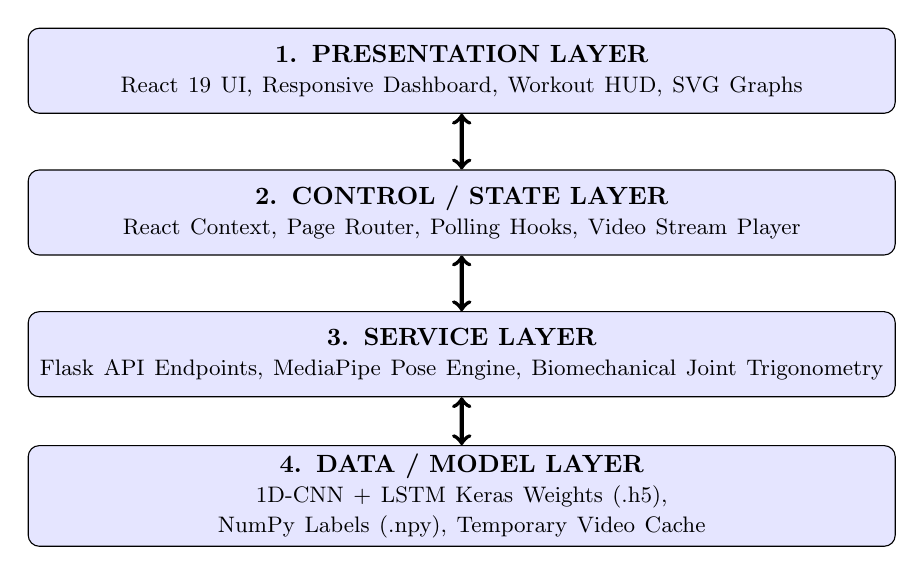
\begin{tikzpicture}[node distance=2cm, scale=0.9, every node/.style={transform shape}]
  % Style definitions
  \tikzstyle{layer} = [rectangle, draw=black, fill=blue!10, text width=12cm, text centered, rounded corners, minimum height=1.2cm, font=\bfseries]
  
  % Layers
  \node (pres) [layer] {1. PRESENTATION LAYER \\ \textnormal{\small React 19 UI, Responsive Dashboard, Workout HUD, SVG Graphs}};
  \node (ctrl) [layer, below of=pres] {2. CONTROL / STATE LAYER \\ \textnormal{\small React Context, Page Router, Polling Hooks, Video Stream Player}};
  \node (serv) [layer, below of=ctrl] {3. SERVICE LAYER \\ \textnormal{\small Flask API Endpoints, MediaPipe Pose Engine, Biomechanical Joint Trigonometry}};
  \node (data) [layer, below of=serv] {4. DATA / MODEL LAYER \\ \textnormal{\small 1D-CNN + LSTM Keras Weights (.h5), NumPy Labels (.npy), Temporary Video Cache}};
  
  % Arrows
  \draw[line width=1.5pt, <->] (pres) -- (ctrl);
  \draw[line width=1.5pt, <->] (ctrl) -- (serv);
  \draw[line width=1.5pt, <->] (serv) -- (data);
\end{tikzpicture}
\caption{Four-Layered System Architecture Diagram.}
\label{fig:system_architecture}
\end{figure}

The responsibilities of the primary components are outlined in Table 3.2:
\begin{table}[h]
\centering
\begin{tabular}{|p{4.5cm}|p{11.3cm}|}
\hline
\textbf{Component} & \textbf{Responsibility} \\ \hline
React App UI (\texttt{App.jsx}) & Layout routing, header navigation, dark-mode glassmorphism rendering. \\ \hline
Workout Studio (\texttt{Playground.jsx}) & Captures camera input, polls FPS and status, renders the live video stream. \\ \hline
Flask Server (\texttt{main.py}) & Establishes API endpoints, handles camera/video frame processing, streams MJPEG responses. \\ \hline
Pose Evaluator (\texttt{body\_part\_angle.py}) & Processes landmarks coordinates to compute mathematical angles. \\ \hline
Repetition Counter (\texttt{types\_of\_exercise.py}) & Keeps track of UP/DOWN movement state cycles to count repetitions. \\ \hline
Sequence Classifier (\texttt{models}) & Classifies workout activities dynamically from 30-frame sequence keypoints. \\ \hline
\end{tabular}
\caption{System Component Responsibilities.}
\label{tab:component_responsibilities}
\end{table}

\section{Proposed Deep Learning Model Architecture}
To classify workout sequences, the system integrates a hybrid deep learning model combining a One-Dimensional Convolutional Neural Network (1D-CNN) and Long Short-Term Memory (LSTM).
\begin{table}[h]
\centering
\begin{tabular}{|p{4.0cm}|p{11.8cm}|}
\hline
\textbf{Parameter} & \textbf{Value / Configuration} \\ \hline
Input Shape & $(30, 132)$ -- 30 sequential frames, each with 132 coordinates (33 landmarks $\times$ 4 features: $x, y, z, \text{visibility}$) \\ \hline
First Layer & Conv1D ($64$ filters, kernel size $3$, activation `relu') \\ \hline
Second Layer & MaxPool1D (pool size $2$) \\ \hline
Third Layer & LSTM ($64$ units, return sequences `false') \\ \hline
Fourth Layer & Dense ($32$ units, activation `relu', dropout $0.2$) \\ \hline
Output Layer & Dense ($13$ classes, activation `softmax') \\ \hline
\end{tabular}
\caption{1D-CNN + LSTM Model Configuration.}
\label{tab:model_config}
\end{table}

\section{End-to-End Processing Workflow}
The workflow of frame processing is structured as follows:
\begin{enumerate}
    \item The camera captures a raw frame and sends it to the Flask server (or processed locally via OpenCV).
    \item The image is converted from BGR to RGB.
    \item MediaPipe processes the frame, returning coordinates for 33 body joints.
    \item The coordinates are extracted, flattened, and added to a 30-frame sequence buffer.
    \item The hybrid model classifies the sequence to predict the active exercise (e.g., squat).
    \item Mathematical formulas calculate the relevant joint angles (e.g., knee flex angle).
    \item The state machine checks thresholds: if angle drops below $70^{\circ}$ and then extends past $160^{\circ}$, it increments the rep counter.
    \item Pose correction checks for alignment warnings (hip sagging, shoulders uneven).
    \item Skeletons, text overlays, and progress bars are drawn onto the frame using OpenCV.
    \item The final frame is JPEG-compressed and streamed back to the React UI as an MJPEG block.
\end{enumerate}

\section{UML Diagrams}

\subsection{System Use Case Diagram}
The actor (User / Athlete) interacts with the system through the React web interface to choose exercises, configure target repetitions, view webcam feedback, or upload videos for analysis.

\begin{figure}[h]
\centering
\begin{tikzpicture}[scale=0.8, every node/.style={transform shape}]
  % Actor
  \draw[line width=1.5pt] (-3,0) circle (0.4); % head
  \draw[line width=1.5pt] (-3,-0.4) -- (-3,-1.6); % body
  \draw[line width=1.5pt] (-3.6,-0.8) -- (-2.4,-0.8); % arms
  \draw[line width=1.5pt] (-3,-1.6) -- (-3.5,-2.5); % left leg
  \draw[line width=1.5pt] (-3,-1.6) -- (-2.5,-2.5); % right leg
  \node[font=\bfseries] at (-3,-3.0) {Athlete / User};
  
  % Use Cases
  \tikzstyle{uc} = [ellipse, draw=black, fill=blue!5, minimum width=4cm, minimum height=1cm, text centered]
  \node (uc1) at (3,2) [uc] {Start Live Workout};
  \node (uc2) at (3,0.7) [uc] {Upload Workout Video};
  \node (uc3) at (3,-0.6) [uc] {Select Exercise Profile};
  \node (uc4) at (3,-1.9) [uc] {View Biomechanical Form};
  
  % System Boundaries
  \draw[line width=1pt, dashed] (0,-3.2) rectangle (6,3.2);
  \node[font=\tiny] at (3,3.0) {CNN - FitnessTracker};
  
  % Relationships
  \draw[line width=1pt, ->] (-2.2,-0.5) -- (uc1.west);
  \draw[line width=1pt, ->] (-2.2,-0.7) -- (uc2.west);
  \draw[line width=1pt, ->] (-2.2,-0.9) -- (uc3.west);
  \draw[line width=1pt, ->] (-2.2,-1.1) -- (uc4.west);
\end{tikzpicture}
\caption{System Use Case Diagram.}
\label{fig:use_case_diagram}
\end{figure}

\newpage
\subsection{Class Diagram}
The core modules and classes of the system:
\begin{figure}[h]
\centering
\begin{tikzpicture}[scale=0.78, every node/.style={transform shape}]
  \tikzstyle{classbox} = [rectangle, draw=black, fill=gray!10, text width=7.5cm, rounded corners, font=\ttfamily\small]
  
  \node (bpa) [classbox] {
    \textbf{BodyPartAngle} \\
    \hline
    + landmarks: List \\
    \hline
    + angle\_left\_arm(): float \\
    + angle\_right\_arm(): float \\
    + angle\_left\_leg(): float \\
    + angle\_right\_leg(): float \\
    + angle\_abdomen(): float \\
    + angle\_plank(): float
  };
  
  \node (toe) [classbox, below of=bpa, node distance=5.5cm] {
    \textbf{TypeOfExercise} (Inherits BodyPartAngle) \\
    \hline
    \hline
    + push\_up(counter, status): list \\
    + pull\_up(counter, status): list \\
    + squat(counter, status): list \\
    + plank(counter, status): list \\
    + calculate\_exercise(ex, cnt, stat): list \\
    + is\_valid\_posture(ex): bool
  };
  
  \draw[line width=1.5pt, <-] (bpa.south) -- (toe.north) node[midway, right] {Inherits};
\end{tikzpicture}
\caption{Core System Class Diagram.}
\label{fig:class_diagram}
\end{figure}

\subsection{Sequence Diagram}
The interaction flow between the client browser, React app, Flask server, and MediaPipe during real-time webcam exercise tracking:

\begin{figure}[h]
\centering
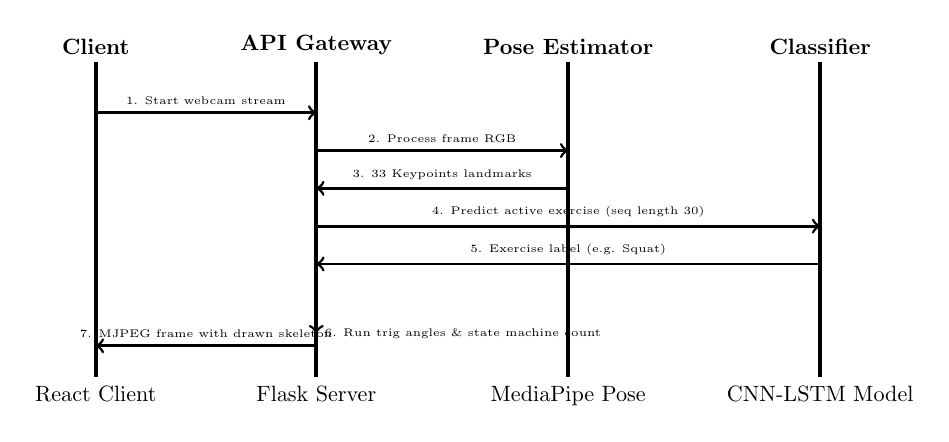
\begin{tikzpicture}[scale=0.8, every node/.style={transform shape}]
  % Lifelines
  \draw[line width=1.5pt] (0,5) -- (0,0) node[below] {React Client};
  \draw[line width=1.5pt] (3.5,5) -- (3.5,0) node[below] {Flask Server};
  \draw[line width=1.5pt] (7.5,5) -- (7.5,0) node[below] {MediaPipe Pose};
  \draw[line width=1.5pt] (11.5,5) -- (11.5,0) node[below] {CNN-LSTM Model};
  
  % Labels
  \node[above, font=\bfseries] at (0,5) {Client};
  \node[above, font=\bfseries] at (3.5,5) {API Gateway};
  \node[above, font=\bfseries] at (7.5,5) {Pose Estimator};
  \node[above, font=\bfseries] at (11.5,5) {Classifier};

  % Messages
  \draw[->, line width=1pt] (0,4.2) -- (3.5,4.2) node[midway, above, font=\tiny] {1. Start webcam stream};
  \draw[->, line width=1pt] (3.5,3.6) -- (7.5,3.6) node[midway, above, font=\tiny] {2. Process frame RGB};
  \draw[<-, line width=1pt] (3.5,3.0) -- (7.5,3.0) node[midway, above, font=\tiny] {3. 33 Keypoints landmarks};
  \draw[->, line width=1pt] (3.5,2.4) -- (11.5,2.4) node[midway, above, font=\tiny] {4. Predict active exercise (seq length 30)};
  \draw[<-, line width=1pt] (3.5,1.8) -- (11.5,1.8) node[midway, above, font=\tiny] {5. Exercise label (e.g. Squat)};
  \draw[->, line width=1pt] (3.5,1.2) -- (3.5,0.7) node[right, font=\tiny] {6. Run trig angles \& state machine count};
  \draw[<-, line width=1pt] (0,0.5) -- (3.5,0.5) node[midway, above, font=\tiny] {7. MJPEG frame with drawn skeleton};
\end{tikzpicture}
\caption{System Inter-Module Sequence Diagram.}
\label{fig:sequence_diagram}
\end{figure}

\section{Software Requirements Specification}

\subsection{Functional Requirements}
\begin{table}[h]
\centering
\begin{tabular}{|p{1.2cm}|p{3.8cm}|p{10.8cm}|}
\hline
\textbf{ID} & \textbf{Requirement} & \textbf{Description} \\ \hline
FR-1 & Stream Camera & The system shall stream live webcam frames to the backend at 640x360 resolution for low-latency computation. \\ \hline
FR-2 & Landmark Tracking & The system shall detect 33 skeletal landmarks in 3D coordinate spaces with visibility scores. \\ \hline
FR-3 & Auto-detect Activity & The sequence classification model shall predict active exercise profiles from the moving sequence. \\ \hline
FR-4 & Joint Trigonometry & The system shall calculate biomechanical angles dynamically based on active exercise rules. \\ \hline
FR-5 & Rep Counting & The system shall count repetitions using DOWN/UP state cycles and prevent double counting via a time-based refractory filter ($0.9$ seconds minimum). \\ \hline
FR-6 & Video Upload & The system shall allow users to upload MP4/AVI videos and output processed video feeds. \\ \hline
\end{tabular}
\caption{System Functional Requirements.}
\label{tab:functional_requirements}
\end{table}

\subsection{Non-Functional Requirements}
\begin{table}[h]
\centering
\begin{tabular}{|p{1.5cm}|p{3.8cm}|p{10.5cm}|}
\hline
\textbf{ID} & \textbf{Requirement} & \textbf{Description} \\ \hline
NFR-1 & Performance & The backend frame processing latency shall be under $16$ milliseconds per frame to support $60$ FPS feeds. \\ \hline
NFR-2 & Local Execution & Landmark tracking must run locally on the client/edge backend thread to ensure zero external API dependencies. \\ \hline
NFR-3 & UI Responsiveness & The React frontend layout must adjust dynamically across mobile, tablet, and desktop screens. \\ \hline
NFR-4 & Accuracy & The exercise sequence recognition accuracy must exceed $95\%$ under normal indoor lighting. \\ \hline
\end{tabular}
\caption{System Non-Functional Requirements.}
\label{tab:non_functional_requirements}
\end{table}

\subsection{Hardware and Software Requirements}
The tables below list the workstation environment specs used during development:
\begin{table}[h]
\centering
\begin{tabular}{|p{4.0cm}|p{11.8cm}|}
\hline
\textbf{Component} & \textbf{Hardware Specification} \\ \hline
Processor & Intel Core i5 / AMD Ryzen 5 or higher \\ \hline
Memory & 8 GB RAM minimum (16 GB recommended) \\ \hline
Video Input & High Definition Webcam (720p or 1080p, 30 FPS minimum) \\ \hline
GPU & Integrated Graphics or Dedicated NVIDIA GeForce card \\ \hline
\end{tabular}
\caption{Development Hardware Requirements.}
\label{tab:hardware_reqs}
\end{table}

\begin{table}[h]
\centering
\begin{tabular}{|p{4.0cm}|p{11.8cm}|}
\hline
\textbf{Component} & \textbf{Software / Library Package Specification} \\ \hline
Operating System & Windows 10/11, macOS, or Ubuntu Linux (64-bit) \\ \hline
Languages & Python 3.9+ and JavaScript (ES6+) \\ \hline
Backend Framework & Flask 2.2.3, Flask-CORS \\ \hline
Computer Vision & OpenCV (opencv-python) 4.7.0, Google MediaPipe 0.9.3 \\ \hline
Deep Learning & TensorFlow/Keras 2.11.0, NumPy \\ \hline
Frontend Framework & React 19, Vite, React-Router-DOM \\ \hline
\end{tabular}
\caption{Development Software Requirements.}
\label{tab:software_reqs}
\end{table}
\newpage
